\documentclass{article}

\usepackage[dutch]{babel}
\usepackage[margin=3cm]{geometry}
\usepackage{graphicx}
\usepackage{float}
\usepackage{caption}
\usepackage{hyperref}


\graphicspath{
    {img/}
} 

\newcommand{\bold}[1]{\textbf{#1}}
 
\begin{document}

\begin{titlepage}
    \author{Tuur Vanhoutte}
    \title{Sensors \& Interfacing}
\end{titlepage}

\pagenumbering{gobble}
\maketitle
\newpage
\tableofcontents
\newpage

\pagenumbering{arabic}

\section {Communicatie}
\subsection{Datacommunicatie in IoT}
3 lagen:
\begin{enumerate}
    \item Application Layer
    \item Fog layer
    \item IoT Device Layer
\end{enumerate}

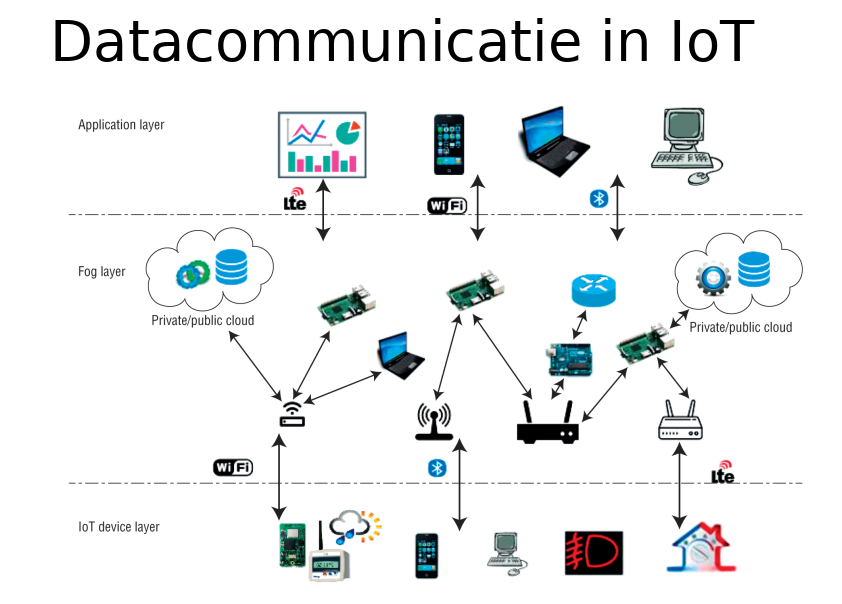
\includegraphics[width=0.95\textwidth]{Screenshot_20200210_120010.png}

\subsection{Data}
\begin{itemize}
    \item "Pre-informatie"
    \item Gegevens waaruit informatie kan worden gewonnen
    \item Stelt een bepaalde toestand voor
\end{itemize}

\subsection{Communicatie}
Overbrengen van informatie tussen deelnemers
\begin{itemize}
    \item Boodschap
    \item Signaal
    \item Medium
\end{itemize}

\subsubsection{Communicatieafspraken}
\begin{itemize}
    \item Coderen van informatie (encoding)
    \item Voorbeeld:
        \item morse-code
        \item Ascii-codering
        \begin{itemize}
            \item Codering voor alle gebruikte symbolen in symbolen
            \item Codering in 7 of 8 bit
            \item 1 byte = 1 teken
        \end{itemize}
        \item \dots
\end{itemize}
  
\subsubsection{Encoding/Decoding}
\begin{enumerate}
    \item Codifying
    \item Sending the message
    \item Decodifying
\end{enumerate}

\subsubsection{Signalen}
\begin{itemize}
    \item Licht
    \item Geluid
    \item Elektriciteit
    \item \dots
\end{itemize}

\subsubsection{Communicatiemedia}
\begin{itemize}
    \item Twisted-Pair cable
    \item Coaxial cable
    \item Fiber-Optic cable
\end{itemize}

\subsubsection{Voorbeelden}
\begin{itemize}
    \item Welke codering?
    \item Wat is het signaal?
    \item Wat is het medium?
\end{itemize}

\subsubsection{Eigenschappen van media}
\begin{itemize}
    \item Vatbaarheid voor interferentie
    \item Overbrugbare afstand
    \item Praktisch
    \item Kostprijs
\end{itemize}

\subsubsection{Afspraken}
\begin{itemize}
    \item Protocol
    \item Standaarden
    \item IEEE
    \item EIA (NEDA/ECA)ECIA
\end{itemize}

\subsubsection{Standaardiseren van \dots}
\begin{itemize}
    \item Type media en zijn specificaties
    \item Het gebruikte signaal en zijn toleranties
    \item De elektrische interferentie
    \item De gebruikte codering
    \item Foutcorrectiecodes
    \item Protocol
    \item De gebruikte connector
    \item \dots
\end{itemize}

\section{Analoog vs digitaal}
\begin{itemize}
    \item \bold{Digitaal}: Discrete waarden
    \item \bold{Analoog}: Continue waarden
\end{itemize}
\subsection{Toestanden}
\subsubsection{Bepaalde toestand}
\begin{itemize}
    \item Temperatuur
    \item Licht aan/uit
    \item Afstand
    \item Tijd
    \item \dots
\end{itemize}

\subsubsection{Digitale toestanden}
\begin{itemize}
    \item Licht aan/uit
    \item Deur open/dicht
    \item Keuze van versnelling N - 1 - 2 - 3 - 4 - 5 - R
    \item Ruitenwisser interval uit - interval - traag - snel
    \item \dots
\end{itemize}

\subsubsection{Analoge toestanden}
\begin{itemize}
    \item Tijd (!)
    \item Temperatuur
    \item Luchtdruk
    \item Luchtvochtigheid
    \item Afstand
    \item \dots
\end{itemize}


\subsection{Signalen}
\begin{itemize}
    \item Analoog signaal
    \item Digitaal signaal
\end{itemize}

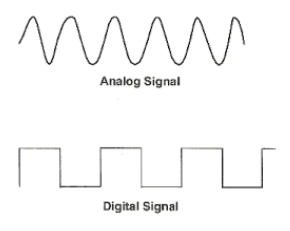
\includegraphics[width=0.4\textwidth]{Screenshot_20200217_115642.png}

\section{Analoge signalen}

\subsubsection{Transducer}
Omzetten van een analoog signaal naar een ander analoog signaal.\\
\bold{Voorbeeld}: elektrisch signaal omzetten naar een geluidsignaal via een luidspreker (=de transducer)

\subsubsection{Sensoren en Actuatoren}
\begin{itemize}
    \item Sensor $\Rightarrow$ meten van een fysieke eigenschap
    \item Actuator $\Rightarrow$ be"invloeden van een fysieke parameter $\Rightarrow$ transducers 
\end{itemize}

\subsection{Analoge communicatie}
Sinusgolf als meest elementaire signaal

\subsubsection{Eigenschappen}
\begin{itemize}
    \item DC vs AC
    \item Polariteit blijft gelijk bij (pulserende) DC
    \item Polariteit verandert bij AC
\end{itemize}

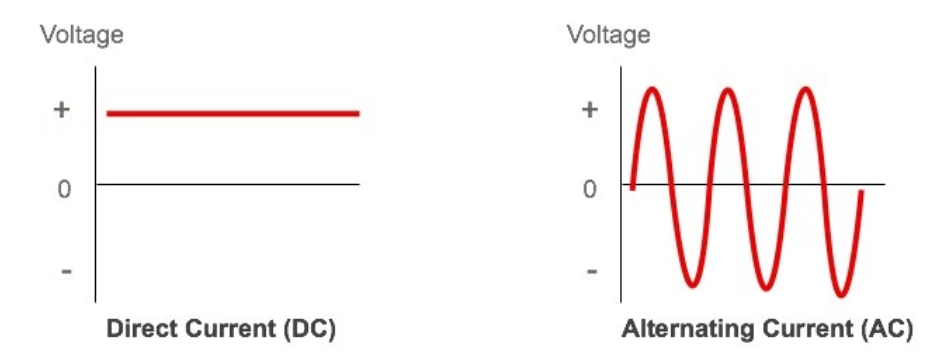
\includegraphics[width=0.5\textwidth]{Screenshot_20200217_121011.png}

\subsubsection{Wisselspanning - Eigenschappen}
\begin{itemize}
    \item RMS = Root Mean Square (= kwadratisch gemiddelde) = effectieve waarde (in geval van sinus)
    \begin{enumerate}
        \item Som van alle kwadraten (= square)
        \item Die som delen door het aantal waardes (= mean)
        \item Neem de vierkantswortel van dat getal
    \end{enumerate}
    \begin{itemize}
        \item Wordt vaak gebruikt in de elektriciteit om het gemiddelde vermogen te vinden
    \end{itemize}
    \item Frequentie
    \item Periode
    \item Amplitude
    \item Peak of top-to-top waarde
\end{itemize}
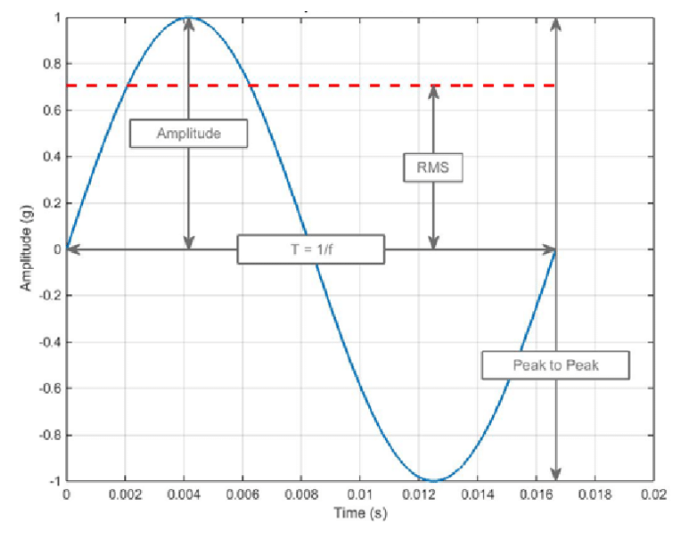
\includegraphics[width=0.7\textwidth]{Screenshot_20200217_121136.png}

\subsubsection{Periodieke signalen}
\begin{itemize}
    \item 1 herhaling = 1 periode
    \item Periode (T) = tijdsduur (in s)
    \item Frequentie (f) = aantal periodes per seconde (in Hz)
    \item $F = \frac1T$ en $T = \frac1F$
\end{itemize}

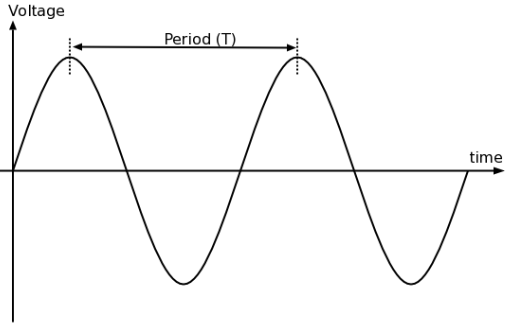
\includegraphics[width=0.7\textwidth]{Screenshot_20200217_122002.png}

\subsubsection{Tijdsdomein en frequentiedomein}
\begin{itemize}
    \item Tijdsdomein: met een oscilloscoop
    \item Frequentiedomein: met 
\end{itemize}

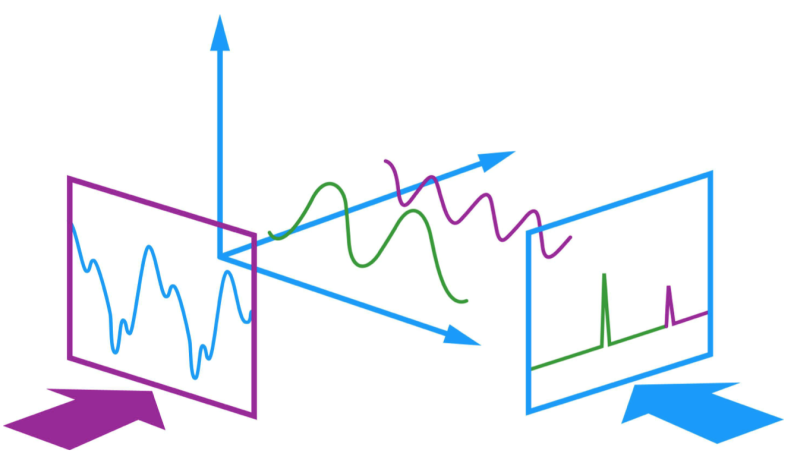
\includegraphics[width=0.7\textwidth]{Screenshot_20200217_122108.png}
\\
(Formule niet te kennen)1
\\
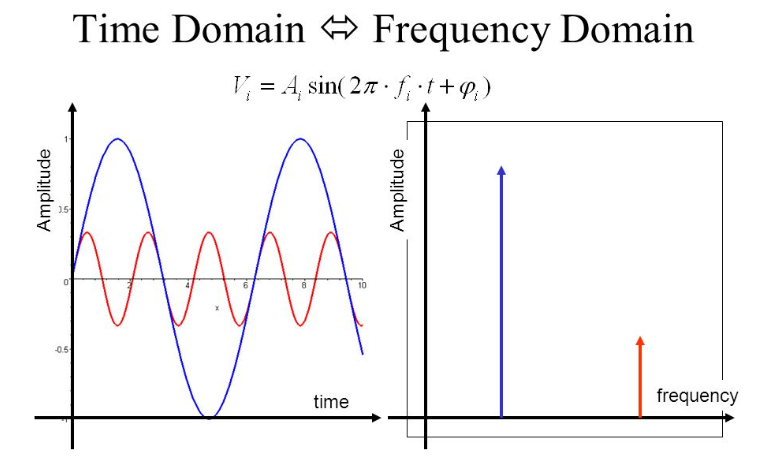
\includegraphics[width=0.7\textwidth]{Screenshot_20200217_122246.png}

\section{Digitale signalen}
Aan/uit


\subsection{Duty Cycle}
= Hoeveel procent van de tijd staat het signaal aan?

\subsection{Flanken (edge)}
\begin{itemize}
    \item Stijgende flank
    \item Dalende flank
    \item Belangrijk bij kloksignalen
\end{itemize}

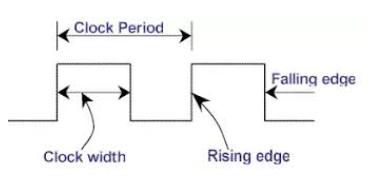
\includegraphics[width=0.5\textwidth]{Screenshot_20200217_123230.png}

\subsection{Weergave digitale signalen}
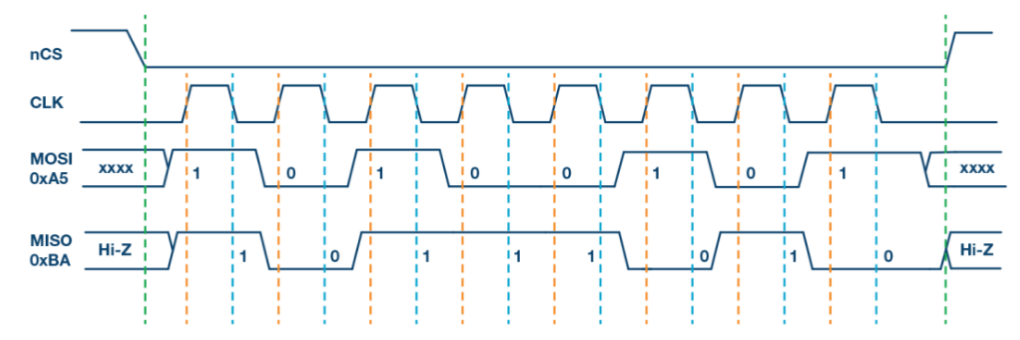
\includegraphics[width=1\textwidth]{Screenshot_20200217_125726.png}

\section{AD/DA conversie}

\begin{figure}[H]
    \centering
    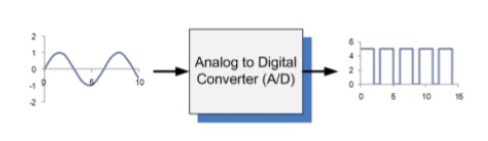
\includegraphics[width=0.7\textwidth]{Screenshot_20200224_115204.png}
    \caption{Analoog naar digitaal (AD converter)}
\end{figure}

\begin{figure}[H]
    \centering
    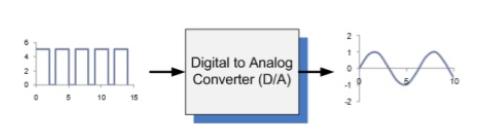
\includegraphics[width=0.7\textwidth]{Screenshot_20200224_115212.png}
    \caption{Digitaal naar analoog (DA converter)}
\end{figure}

\subsection{Analoog naar digitaal}

\begin{figure}[H]
    \centering
    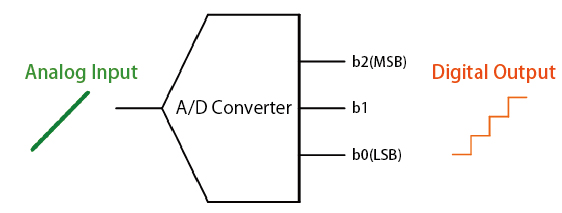
\includegraphics[width=0.7\textwidth]{Screenshot_20200224_115430.jpg}
    \caption{}
\end{figure}

\begin{itemize}
    \item Range = verschil tussen laagste en hoogste waarde
    \item Resolutie = aantal stappen of stapgrootte in bits
    \item Belangrijk gevolg:
    \begin{itemize}
        \item beide parameters bepalen de exactheid en de afwijkingen
    \end{itemize}
\end{itemize}

\subsubsection{Voorbeeld A}
\begin{itemize}
    \item Range = 2V - 2.5V
    \item Resolutie = 8bits
    \item Dus aantal discrete stappen = $2^8 = 256 \Rightarrow 256 - 1 = 255$
    \item Stapgrootte (LSB) = $\frac{range}{255} = \frac{2.5V - 2V}{255} = \frac{0.5V}{255} = 0.00196..V / stap$
    \item ofwel $\approx$ $2mV$/stap
\end{itemize}


\subsubsection{Voorbeeld B}
\begin{itemize}
    \item Range = 0V - 12V
    \item Resolutie = 12bits
    \item Dus aantal discrete stappen = $2^{12} = 4096 \Rightarrow 4096 - 1 = 4095$
    \item Stapgrootte (LSB) = $\frac{range}{4095} = \frac{12V - 0V}{4095} = \frac{12V}{4095} = 0.0029304..V / stap$
    \item ofwel $\approx$ $3mV$/stap
\end{itemize}


\begin{figure}[H]
    \centering
    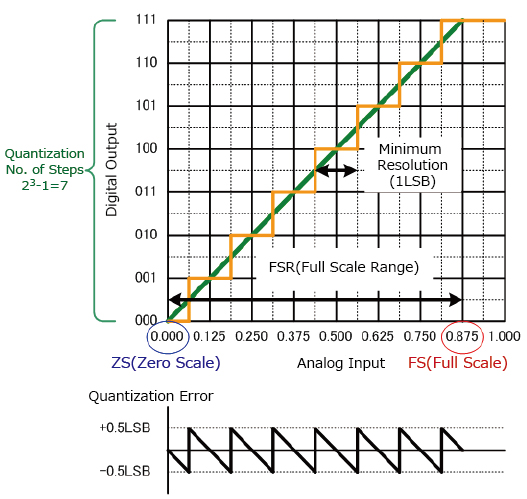
\includegraphics[width=0.7\textwidth]{Screenshot_20200224_120800.jpg}
    \caption{AD conversie}
\end{figure}

\begin{itemize}
    \item Quantisatiefouten
    \item Verzoorzaakt quantisatieruis
\end{itemize}

\begin{figure}[H]
    \centering
    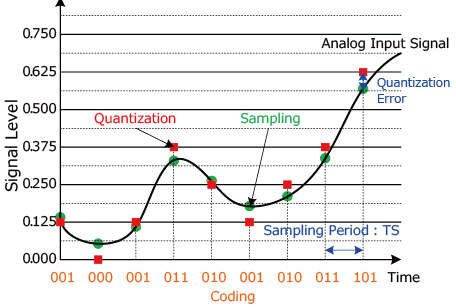
\includegraphics[width=0.7\textwidth]{Screenshot_20200224_120900.jpg}
    \caption{AD conversie}
\end{figure}

\begin{itemize}
    \item Quantisatiefouten $\rightarrow$ dithering
    \item = \underline{vooraf} (witte) ruis toevoegen aan signaal
\end{itemize}

\begin{figure}[H]
    \centering
    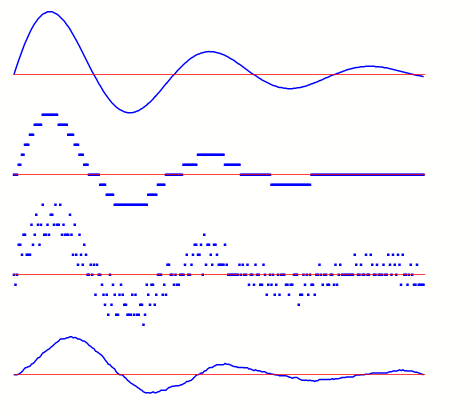
\includegraphics[width=0.7\textwidth]{Screenshot_20200224_121151.png}
    \caption{Dithering}
\end{figure}

\subsubsection{Sample Rate / sample frequentie}
= aantal conversies per seconde
\begin{figure}[H]
    \centering
    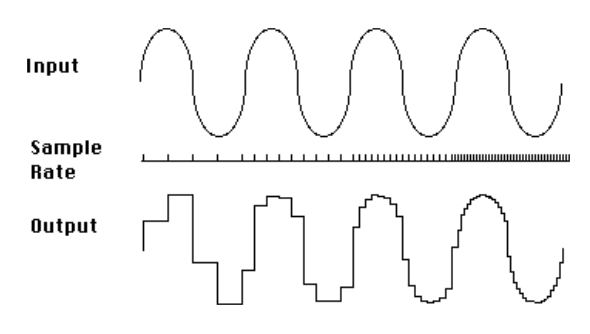
\includegraphics[width=0.7\textwidth]{Screenshot_20200224_121653.png}
    \caption{Sample rate}
\end{figure}

\begin{itemize}
    \item Nyquist $\rightarrow$ Minimale sample rate = 2x de frequentie van het signaal
    \item Voorbeelden:
    \begin{itemize}
        \item HiFi Audio CD: 44.1kHz sample rate
        \item Oude telefoontoestellen: 8kHz sample rate
        \item HD-DVD Audio: 192kHz
    \end{itemize}
\end{itemize}

\begin{figure}[H]
    \centering
    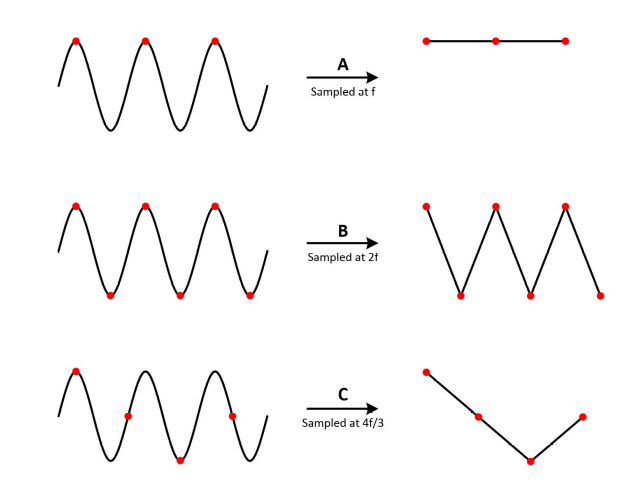
\includegraphics[width=0.7\textwidth]{Screenshot_20200224_121935.png}
    \caption{Minimale sample rate}
\end{figure}

\subsubsection{Aliasing}
= HF signaal als LF 'spooksignaal' detecteren 
\begin{itemize}
    \item Treedt op bij onvoldoende hoge sample rate
    \item Anti-Aliasing filter (low-pass filter) beperkt signaal onder nyquist frequentie
\end{itemize}

\begin{figure}[H]
    \centering
    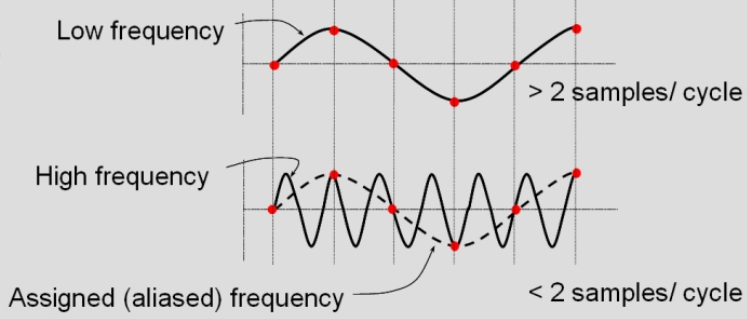
\includegraphics[width=0.7\textwidth]{Screenshot_20200224_122204.png}
    \caption{Anti-aliasing filter}
\end{figure}

\subsubsection{Oversampling}
\begin{itemize}
    \item Sampelen met veelvoud van nyquist frequentie
    \item Kan worden gebruikt om de resolutie op te voeren
    \item Kan worden gebruikt om digitaal (DSP) te filteren
    \item Verhoogt het effectieve aantal bits van de ADC
    \begin{itemize}
        \item \underline{Voorbeeld:} 20bit ADC met 256x OS = 24bit effectieve resolutie
    \end{itemize}
    \item Undersampling $\rightarrow$ specifiek gebruik bij mixers
\end{itemize}

\subsubsection{Implementatie en types}
\begin{itemize}
    \item De comparator
    \item Bekeken als 1-bit ADC
\end{itemize}

\begin{figure}[H]
    \centering
    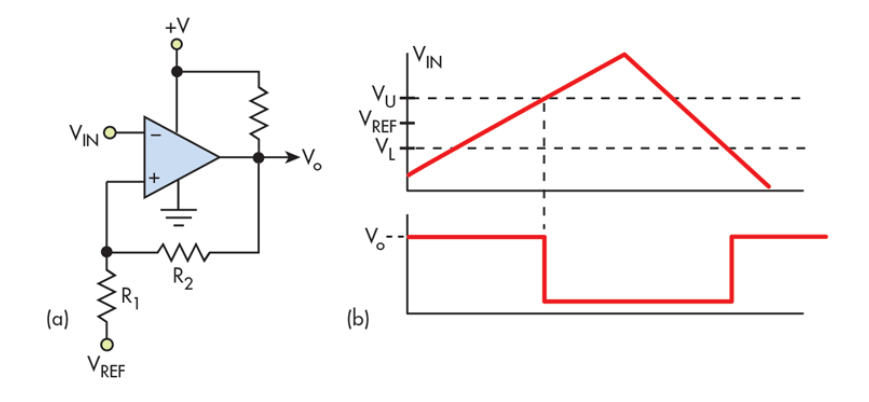
\includegraphics[width=0.7\textwidth]{Screenshot_20200224_122504.png}
    \caption{Comparator}
\end{figure}

\subsubsection{Flash ADC}
\begin{itemize}
    \item Comparator per 'level'
    \item Zeer snel = directe omzetting
    \item Complex \& High power
    \item Lagere resoluties
\end{itemize}

\begin{figure}[H]
    \centering
    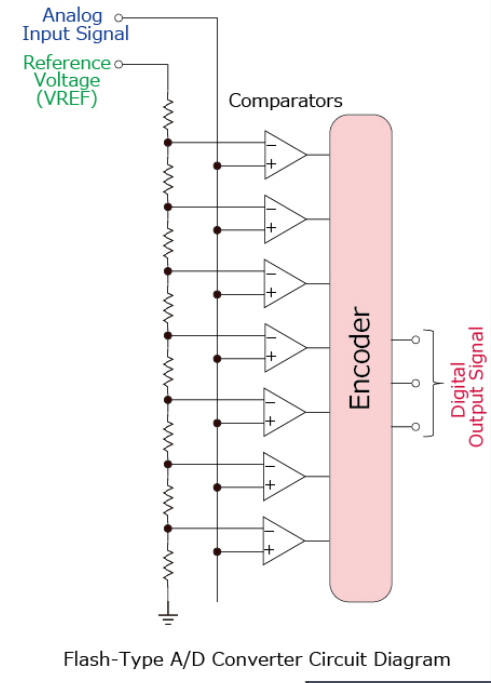
\includegraphics[width=0.7\textwidth]{Screenshot_20200224_122635.png}
    \caption{Flash ADC}
\end{figure}

\subsubsection{Successive approximation ADC}
\begin{itemize}
    \item Gebruikt 1 comparator
    \item Vergelijkt een opgewekte spanning met het signaal
    \item Hoge resolutie mogelijk
    \item Trager
    \item Relatief goedkoop
\end{itemize}

\begin{figure}[H]
    \centering
    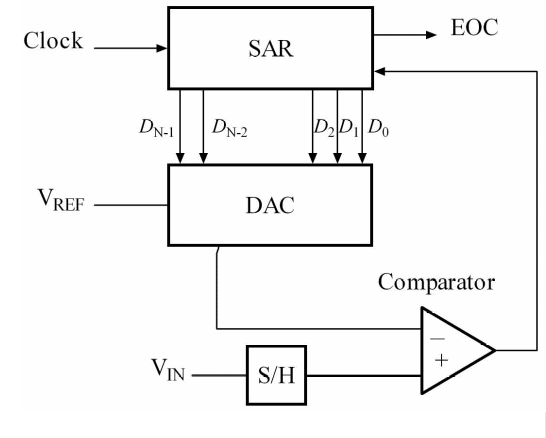
\includegraphics[width=0.7\textwidth]{Screenshot_20200224_122846.png}
    \caption{Successive approximation ADC}
\end{figure}

\subsection{Digitaal naar analoog conversie}
\begin{itemize}
    \item Omzetten digitale naar analoge waarde
    \item Range
    \item Resolutie
    \item Samplefrequentie
\end{itemize}

\subsubsection{Simpele DAC}
\begin{itemize}
    \item Binair $\rightarrow$ analoge waarde
    \item \underline{Voorbeeld} weerstandsnetwerk
\end{itemize}

\begin{figure}[H]
    \centering
    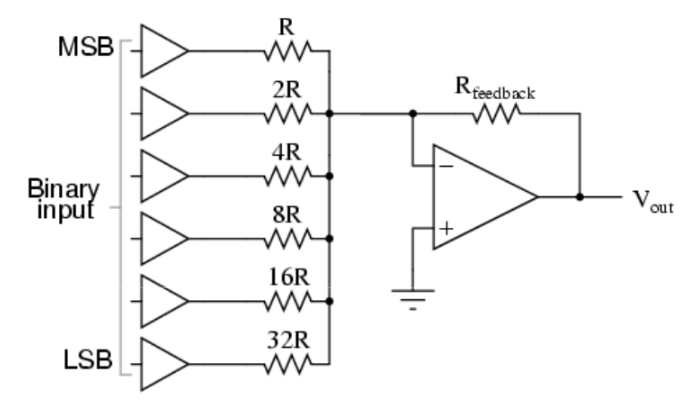
\includegraphics[width=0.7\textwidth]{Screenshot_20200224_123043.png}
    \caption{Weerstandsnetwerk}
\end{figure}

\subsubsection{Simpele DAC adhv PWM}
\begin{itemize}
    \item PWM == digitaal signaal
    \item Door variatie van duty-cycle kan de gemiddelde waarde worden gevarieerd
    \item Door filteren kan de blokgolf worden omgezet in een variabele analoge waarde 
\end{itemize}

\begin{figure}[H]
    \centering
    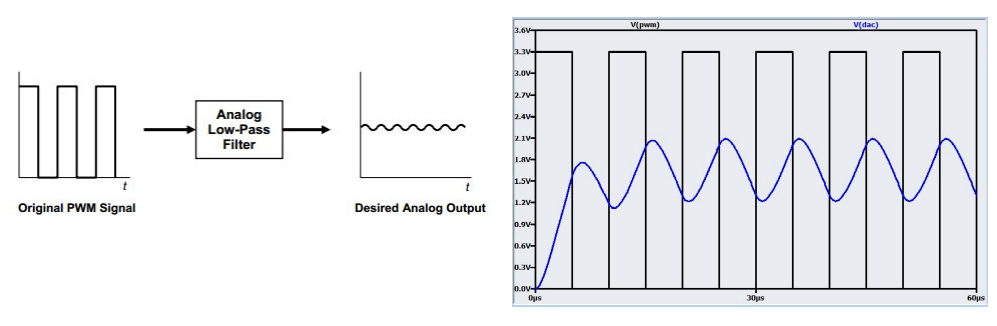
\includegraphics[width=0.7\textwidth]{Screenshot_20200224_123240.png}
    \caption{DAC met PWM}
\end{figure}

\subsubsection{Andere types}
\begin{itemize}
    \item $\Sigma\Delta$
    \item $I^2S$ DAC
    \item Nog zeer veel andere overwegingen:
    \begin{itemize}
        \item THD (Harmonische vervorming)
        \item Faseruis
        \item \dots
    \end{itemize}
\end{itemize}

\subsubsection{Nalezen:}
\begin{itemize}
    \item \url{https://en.wikipedia.org/wiki/Digital-to-analog_converter}
    \item \url{https://en.wikipedia.org/wiki/Analog-to-digital_converter}
    \item \url{https://en.wikipedia.org/wiki/Nyquist%E2%80%93Shannon_sampling_theorem}
    \item \url{https://en.wikipedia.org/wiki/Nyquist_rate}
    \item \url{https://en.wikipedia.org/wiki/Pulse-width_modulation}
    \item \url{https://en.wikipedia.org/wiki/Delta-sigma_modulation}
\end{itemize}



\end{document}
